\documentclass{article}
\usepackage[top=1in, bottom=1.25in, left=1.10in, right=1.10in]{geometry}
\usepackage{amsmath,graphicx,multicol,multirow}

% Example definitions.
% --------------------
\def\x{{\mathbf x}}
\def\L{{\cal L}}

% Title.
% ------
\title{Parallelization of Neural Network Training using Model Averaging and Butterfly Mixing}
%
% Single address.
% ---------------
\author{Hang Su, Haoyu Chen}
\date{}

\begin{document}
%\ninept
%
\maketitle
%
\begin{abstract}
In this work, we introduce Butterfly mixing to parallel training of deep neural networks (DNN). Parallelization is done
in a model averaging manner. Data is partitioned and distributed to different nodes for local model update, and
model averaging (reduce) is done every few minibatches. We compare several different reduce stratgies, including
all-reduce, butterfly mixing, ring reduce. We show that all these methods can effectively
speed up neural network training. On TIMIT data set, a 10x speed up is achieved using 16 gpus when natural gradient
based stochastic gradient descent is used.
\end{abstract}
%
%
\section{Introduction}
\label{sec:intro}
Deep Neural Networks (DNN) has shown its effeciveness in several machine learning tasks, espencially in speech
recognition. The large model size and massive training examples make DNN a powerful model for classification. However,
these two factors also slow down the training procedure of DNNs.

Parallelization of DNN training has been a popular topic since the revive of neural networks. Several different strategies
have been proposed to tackle this problem. Multiple thread CPU parallelization and single CUDA GPU implementation are compared
in \cite{scanzio2010parallel,vesely2010parallel}, and they show that single GPU could beat 8 cores CPU by a factor of 2.

Optimality for parallelization of DNN training was analyzed in \cite{seide2014parallelizability}, and based on the analysis, 
a gradient quantization approach was proposed to minimize communication cost \cite{seide20141}.

DistBelief proposed in \cite{dean2012large} reports a speed up of 2.2x using 8 CPU coresthan using a
single machine. Asynchronous SGD using multiple GPUs achieved a 3.2x speed-up on 4 GPUs \cite{zhang2013asynchronous}.

A pipeline training approach was propoased in \cite{chen2012pipelined} and a 3.3x speedup was achieved using 4 GPUs, but this
method does not scale beyond number of layers in the neural network.

A speedup of 6x to 14x was achieved using 16 GPUs on training convolutional neural networks \cite{coates2013deep}. In this approach,
each GPU is responsible for a partition of the neural network. This approach is more useful for image classification where 
local structure of the neural network could be exploited.

Distributed model averaging using CPUs is proposed in \cite{zhang2014improving},
and a further improvement is done using natural gradient \cite{povey2014parallel}.

Butterfly mixing was proposed in \cite{zhao2013butterfly} to interleave communication with computation.

\section{Data parallelization and Model Averging}
Gradient descent method is applied to train the DNN model even it's a non-convex optimization problem. 
Since the size of training data is large, batch training is applied to approximately compute the 
gradient for each iteration. Rougly, the larger batch size, the higher converge speed. However, 
the large batch size brings the computing time and memory usage problem. With using distributed 
system, the gradient can be computed at each node, communicate among all the nodes, and average 
recieved gradient at each update iteration. This method can compute the reduced gradient 
accurategly, but it requires heavy communication, since we need to communicate at each update iteration.

However, if the weight rather than gradient of weight is choosen to reduce and average, 
it is not necessary to communicate the weight at each iteration. Thus, in this project, 
we choose to communicate the weight for some fixed iterations steps. 

\section{Reduce Strategies}
In this section, the three data reduce strategies are introduced, which are all-reduce, 
butterfly mixing and ring reduce.

\subsection{All-reduce}
All-reduce startegy collects the weights from all the nodes in the network. The communication is bounded by 
the bandwidth. Fig~\ref{fig:allreduce} is an example of all-reduce with 4 nodes. After one node collects all 
the weights, it will average the weights and then boardcast it too all the nodes. Thus, the all-reduce 
requires at least twice communication to collect and boardcast the messages. However, the all-reduce can 
compute the average weight based on full information for the whole network. Thus, the converge speed of 
all-reduce should be the fastest.
\begin{figure}[htb]
  \centering
  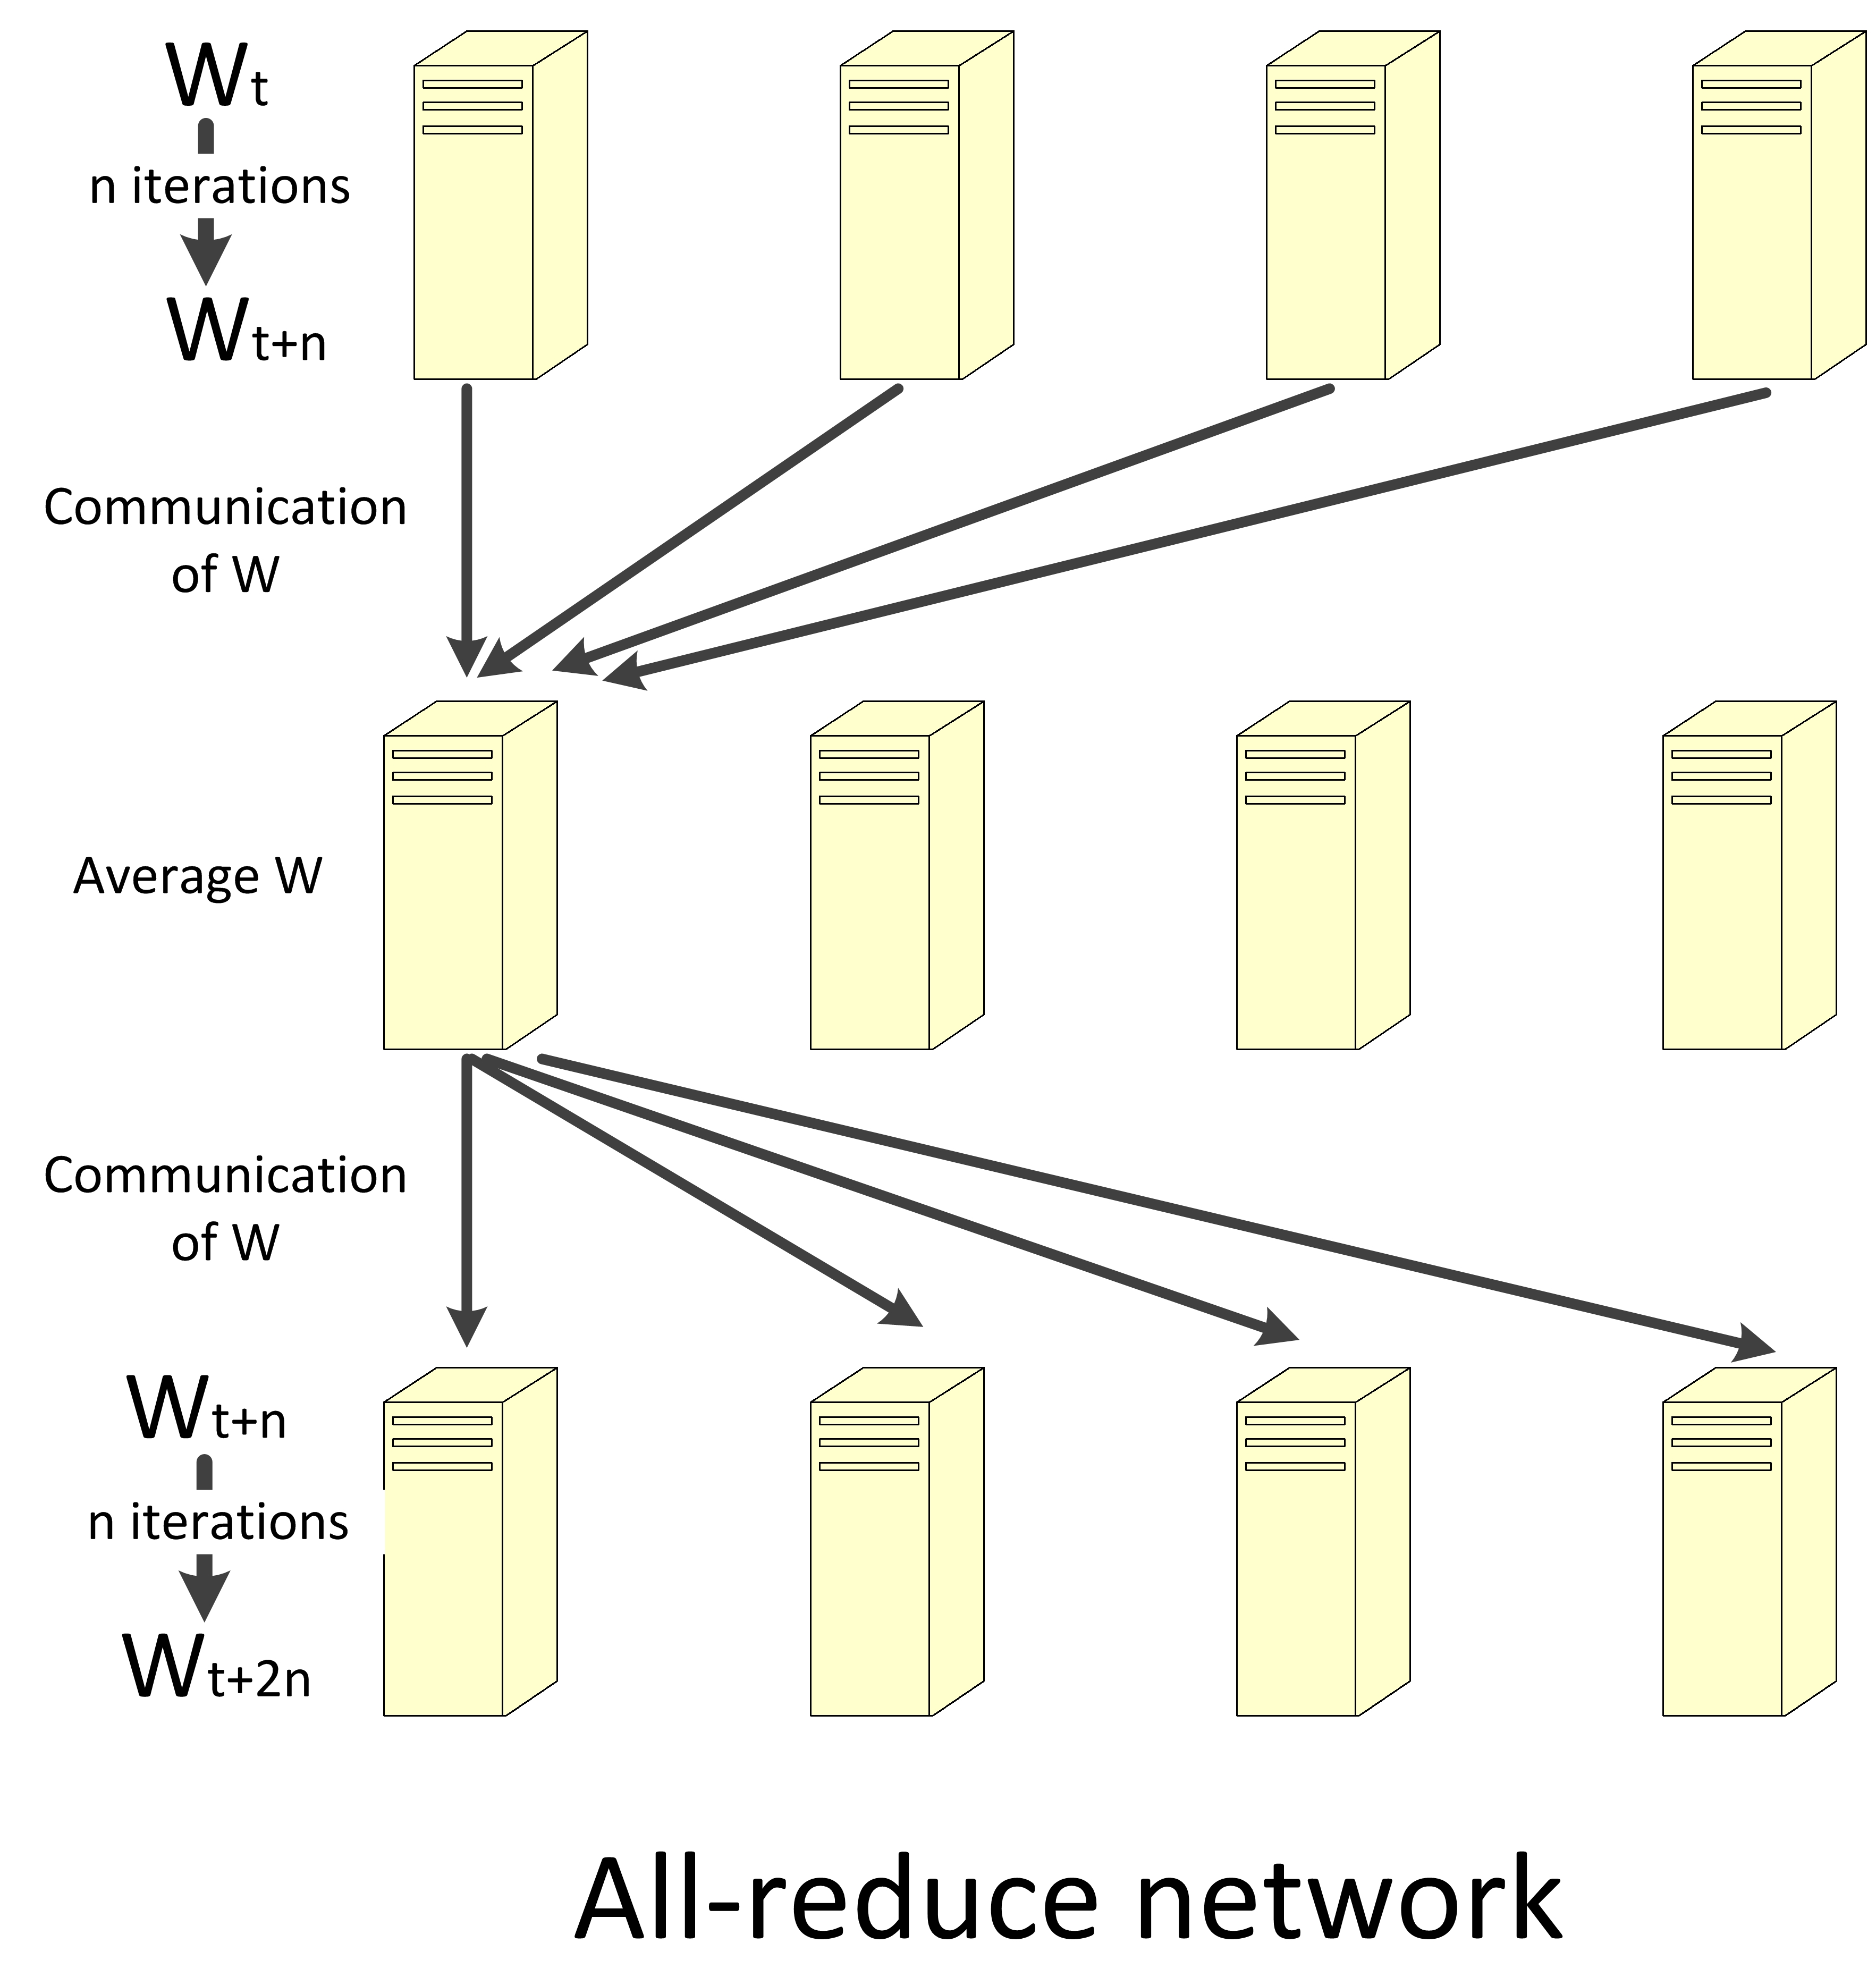
\includegraphics[width=0.5\textwidth]{allreduce.jpg}
  \caption{All-reduce network}
  \label{fig:allreduce}
\end{figure}


\subsection{Butterfly Mixing}
Butterfly mixing a reduction strategy is proposed in \cite{zhao2013butterfly}. It reduces the communication for each 
iteartion: one node would only send and recieve message from one other node, but their communications ensure information 
for the whole network still can be spread to all nodes. Fig~\ref{fig:butterfly} is an example of butterfly mixing with 4 
nodes. The communication of butterfly mixing is bounded by the lantency. And butterfly mixing only require 
once communication to collect and average the weight, it does not need to send the averaged weight. Thus, the 
butterfly mixing has much less communication amount than all-reduce strategy. However, one node at butterfly mixing 
network only collect partial information from the network, its averaged weight can only reflect the information 
from two nodes. It takes $log(number of nodes)$ communication times to spread the message to the whole network. 
Thus, the converge speed of butterfly mixing is slower than all-reduce strategy. 
\begin{figure}[htb]
  \centering
  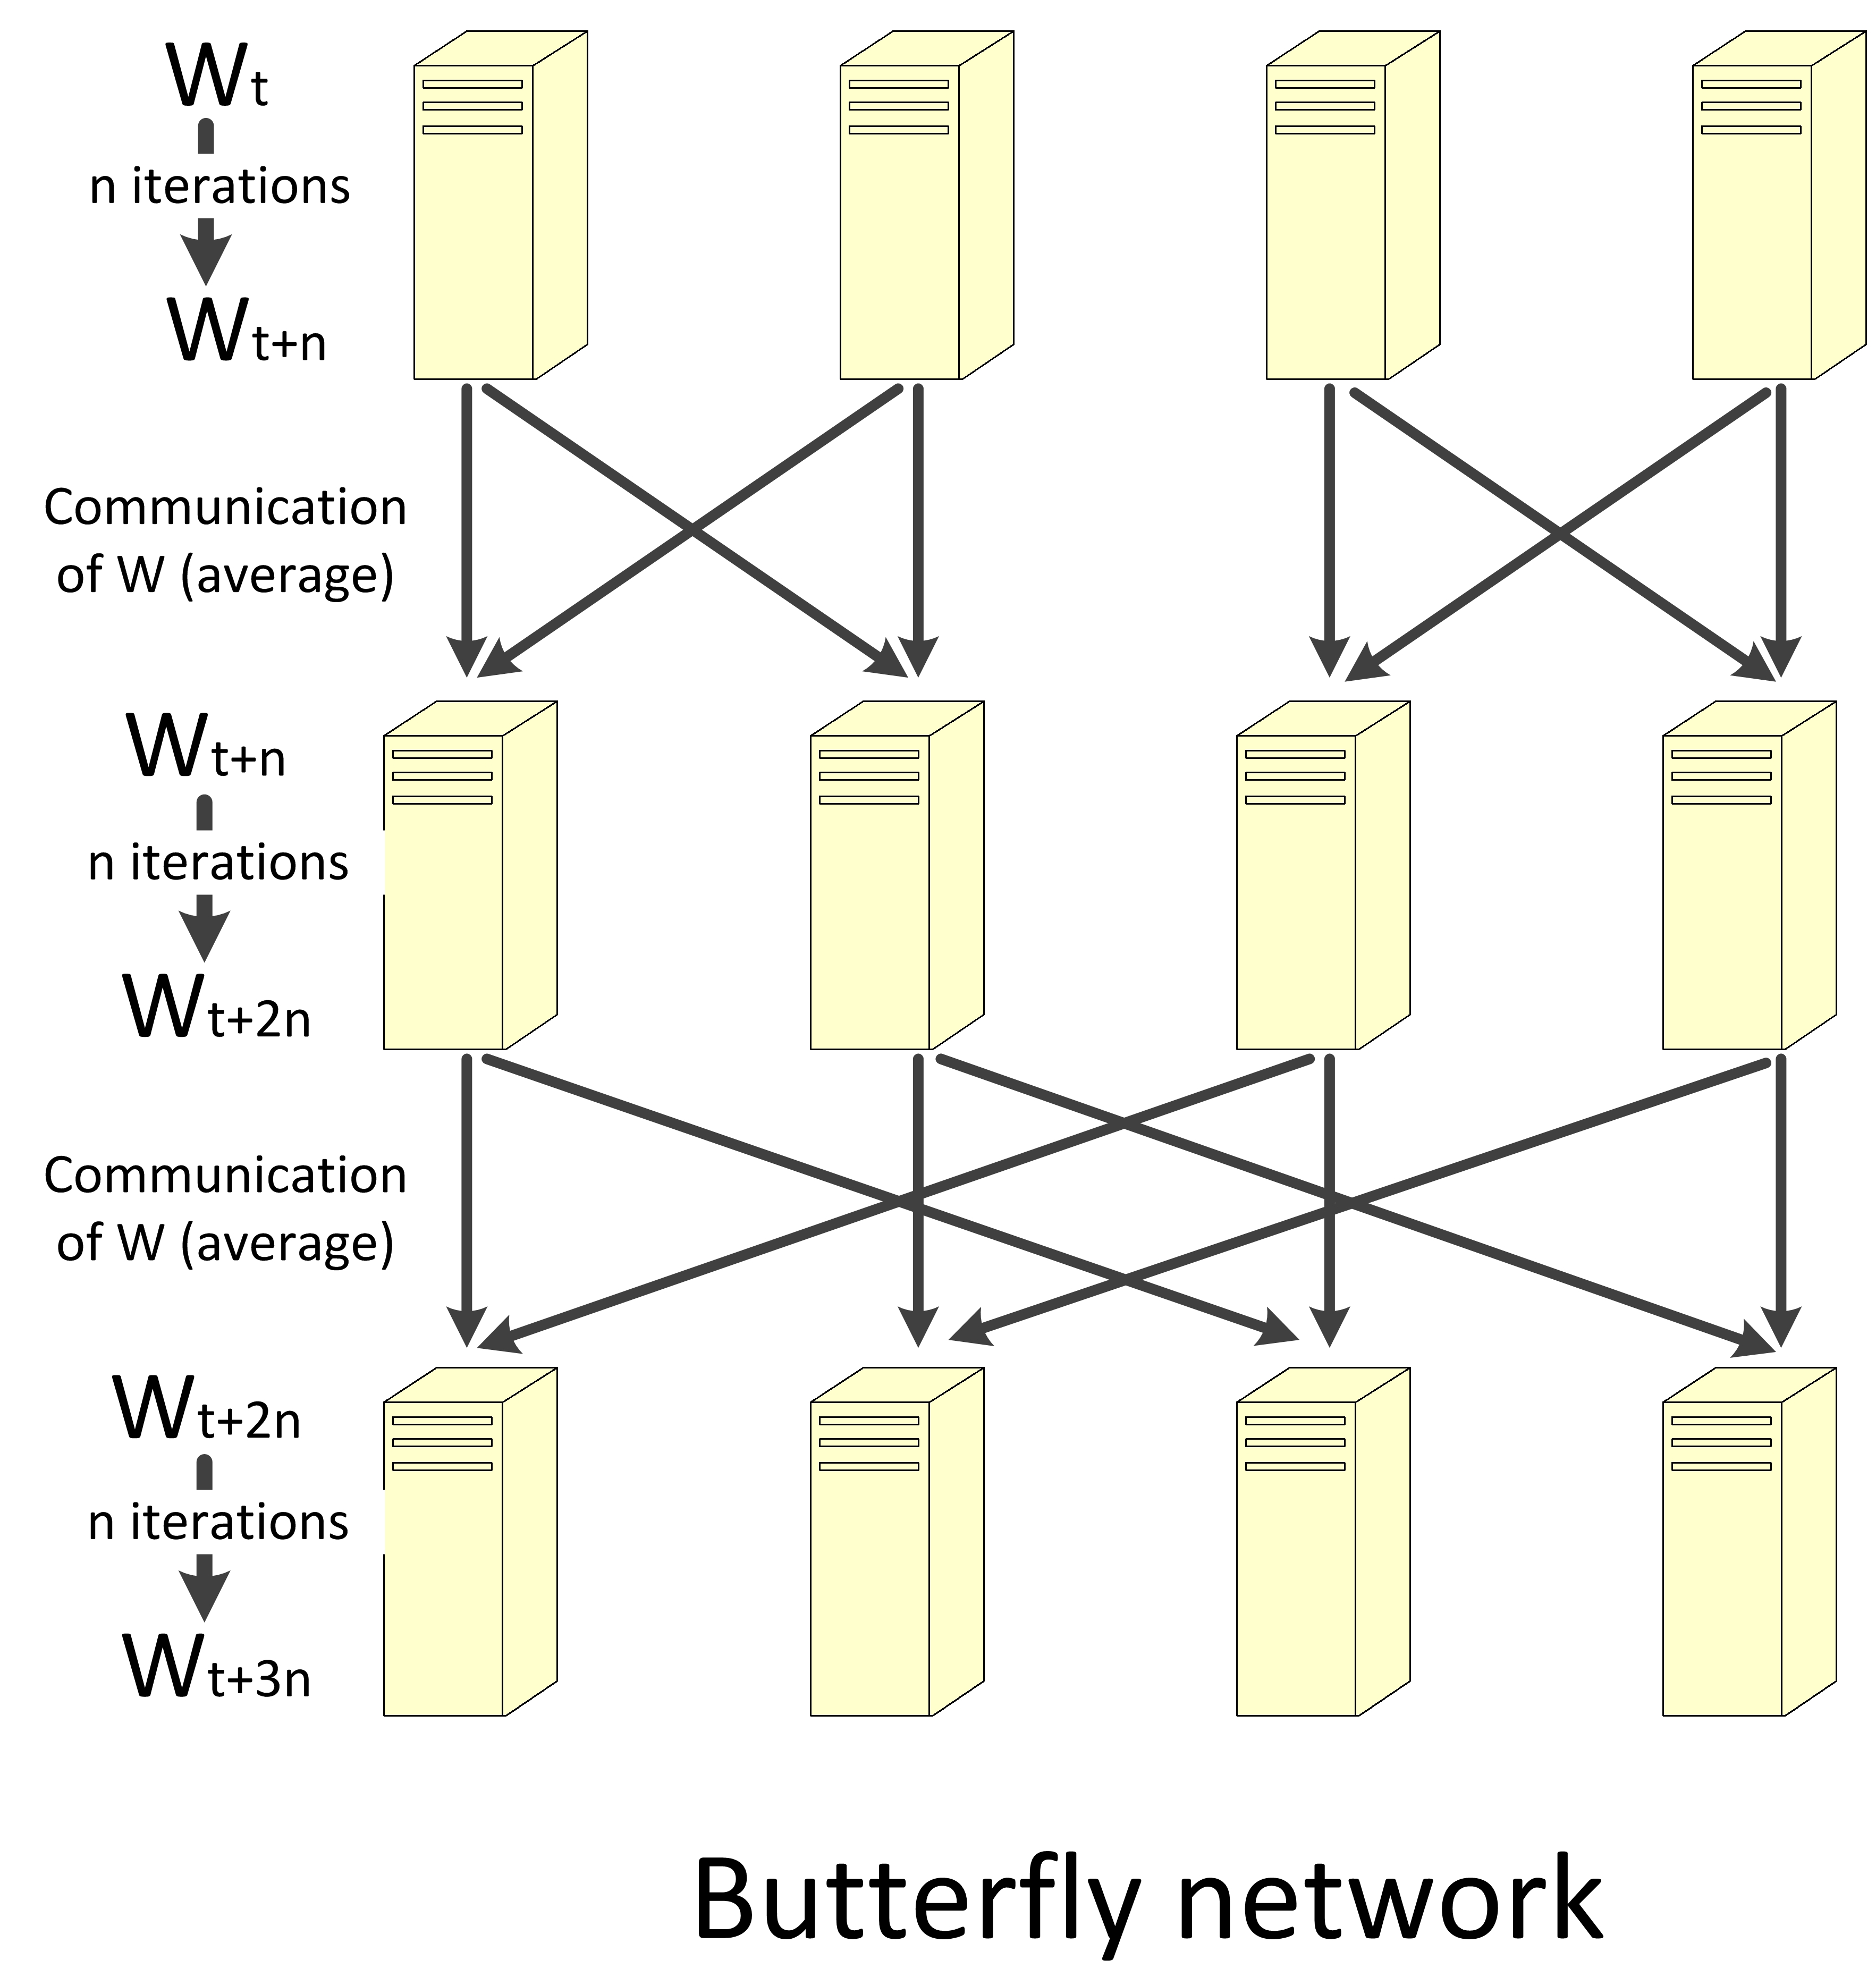
\includegraphics[width=0.5\textwidth]{butterfly.jpg}
  \caption{Butterfly mixing network}
  \label{fig:butterfly}
\end{figure}

\subsection{Ring Reduce}
Each node in ring reduce network would send message to the next node, and receive message from the previous node, 
see Fig~\ref{fig:ring}. Similar as the butterfly mixing, ring network is bounded by the network latency. Ring network also 
only requires once communication to send and collect the weight. However, the ring network requires $number of nodes$ 
communication times to spread the message thoughout the whole network. Thus, the converge speed of 
ring network is the slowest among these three networks. 
\begin{figure}[htb]
  \centering
  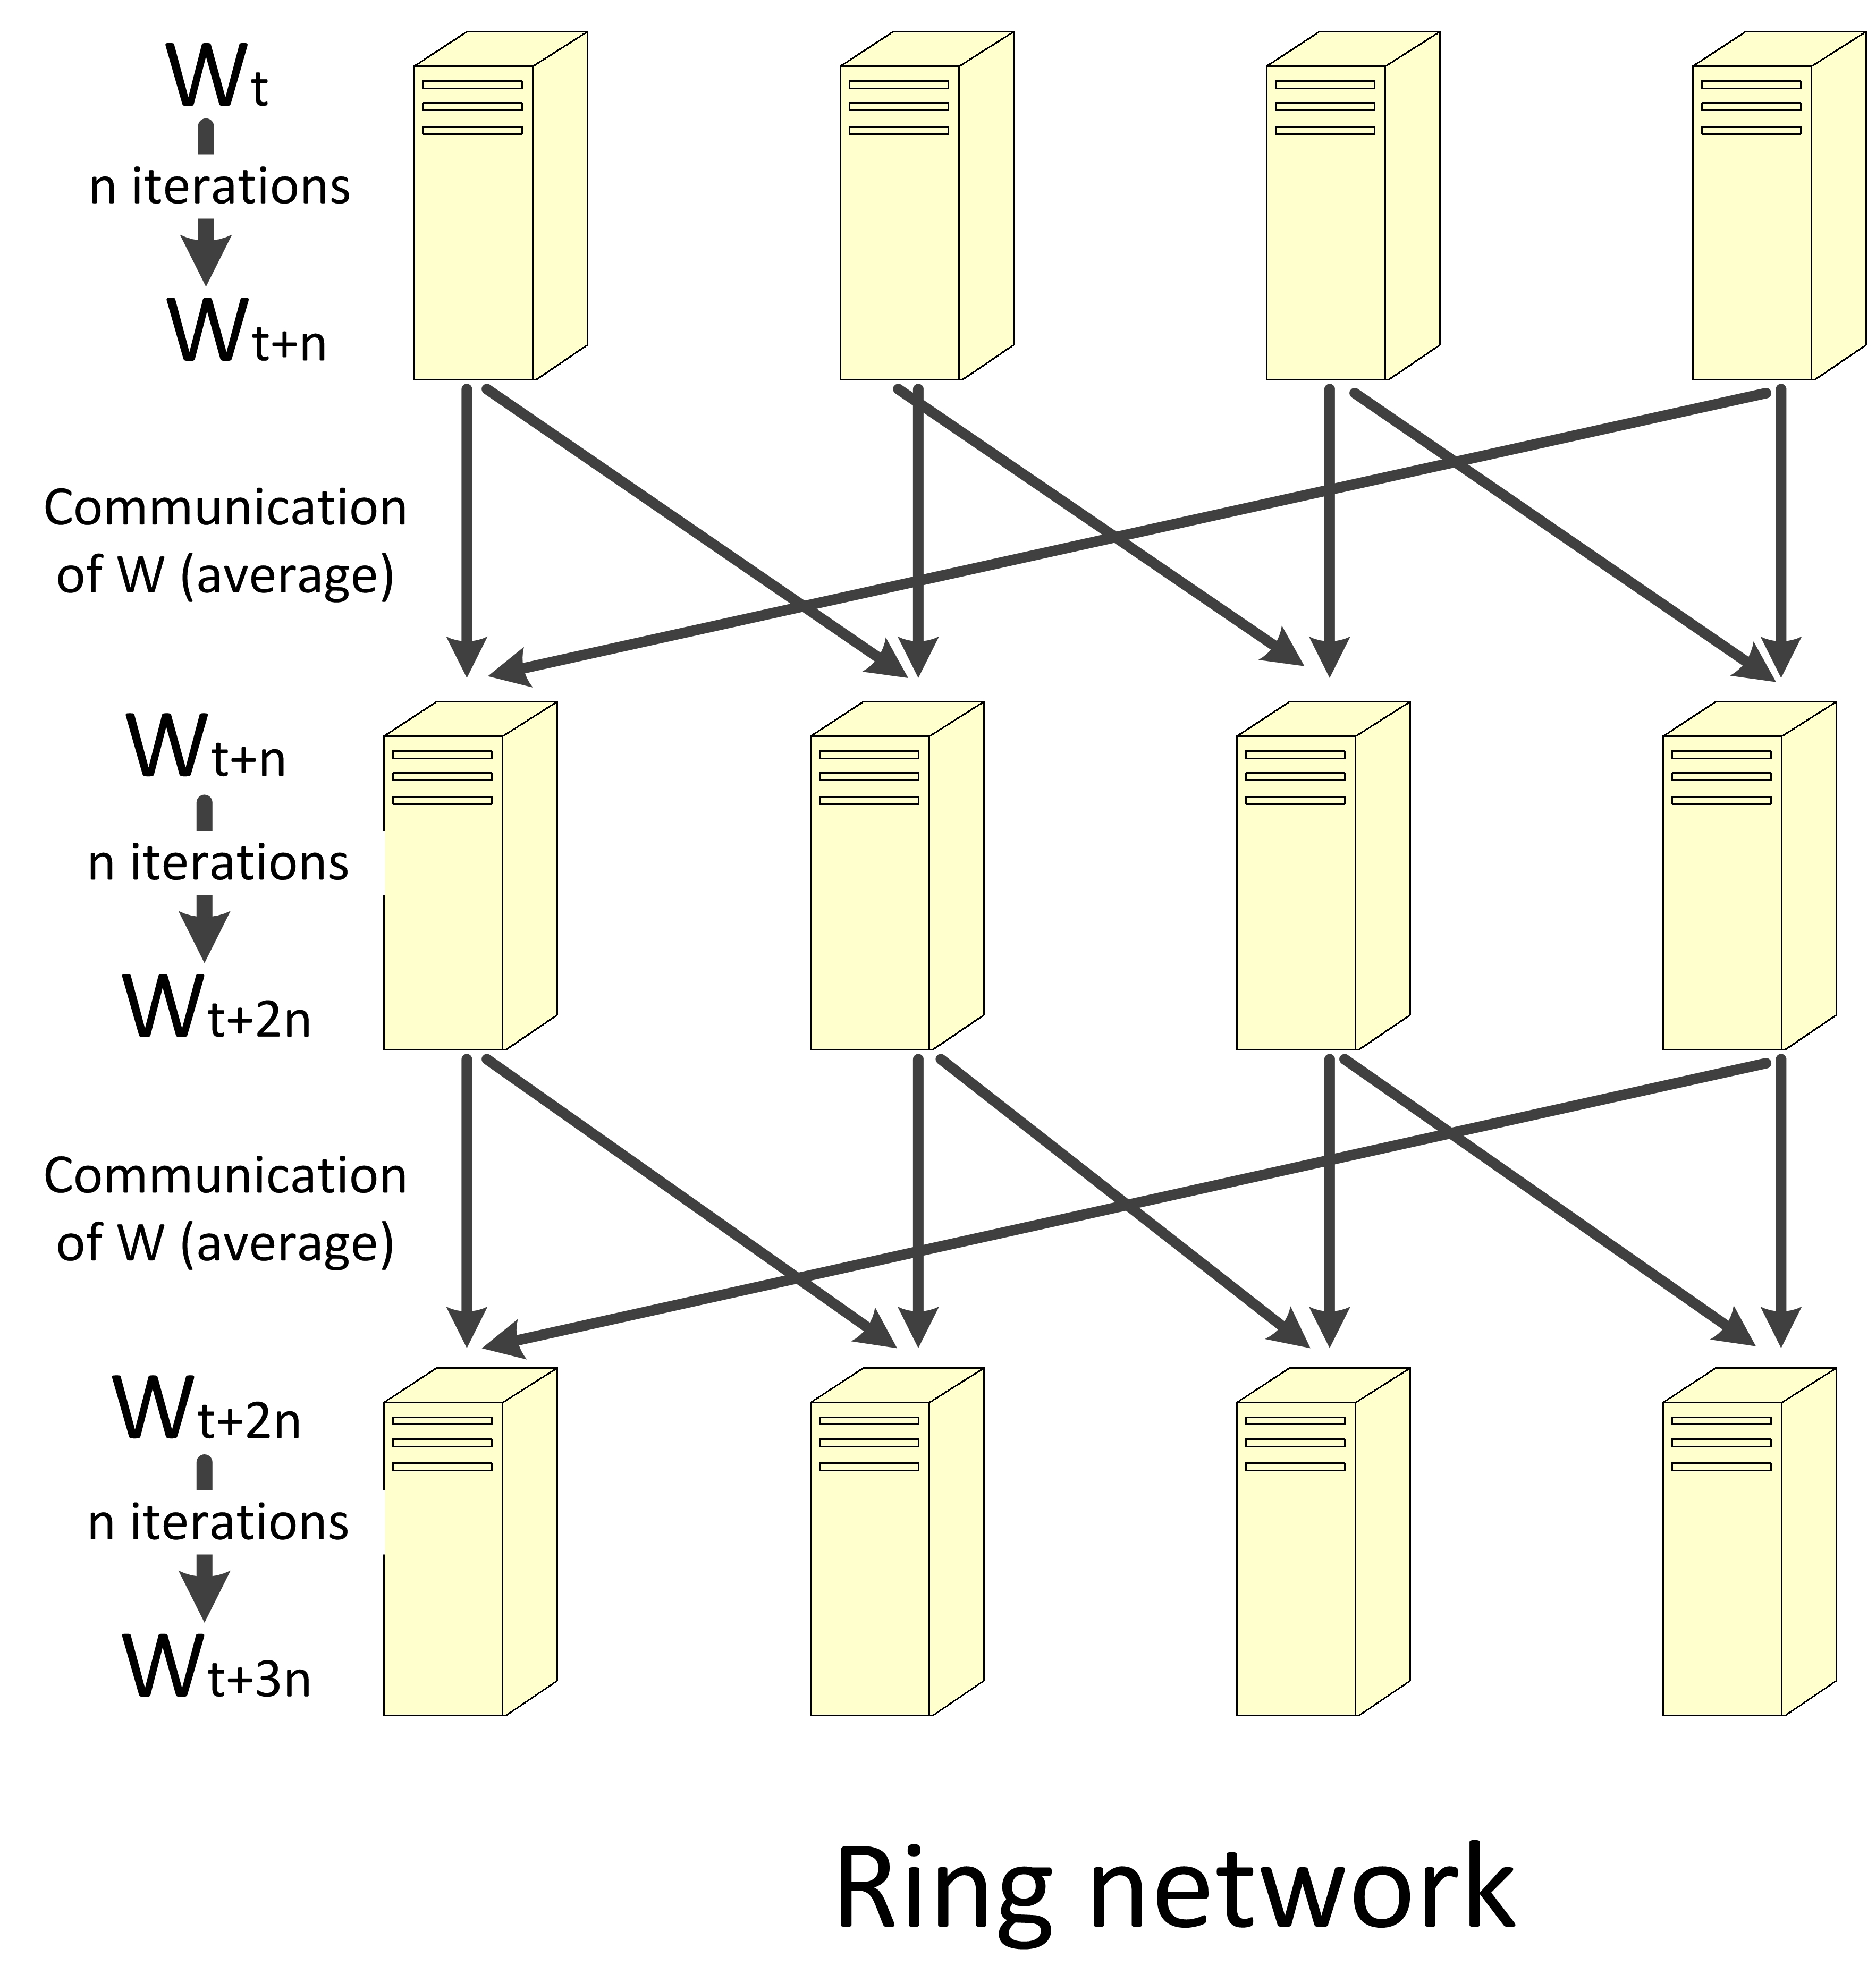
\includegraphics[width=0.5\textwidth]{ring.jpg}
  \caption{Ring network}
  \label{fig:ring}
\end{figure}

\section{Natural Gradient for Model Update}
In stochastic gradient descent (SGD), the learning rate is often assumed to be a scalar $\alpha_t$ that may change over time,
the update formula for model parameters $\theta_{t}$ is
\begin{equation}
\theta_{t+1} = \theta_{t} + \alpha_t g_t
\end{equation}
where $g_t$ is the gradient.

However, according to Natural Graident idea \cite{murata1999statistical,roux2008topmoumoute}, it is possible to replace the scalar with a 
symmetric positive definite matrix $E_t$, which is the inverse of the Fisher information matrix.
\begin{equation}
\theta_{t+1} = \theta_{t} + \alpha_t E_t g_t
\end{equation}

Suppose $x$ is the variable we are modeling, and $f(x;\theta)$ is the probability or likelihood of $x$ given parameters $\theta$, then the
Fisher information matrix $I(\theta)$ is defined as
\begin{equation}
\frac{\partial}{\partial\theta}\log f(x;\theta)
\end{equation}

For large scale speech recognition, it is impossible to estimate Fisher information matrix and perform inversion, so it is necessary to 
approximate the inverse Fisher information matrix directly. We do not include too much detail here because this is not the main focus 
in this report. Details about implementation of NG-SGD could be found in \cite{povey2014parallel}.

\section{Experiments}
\subsection{Setup}
Experiments are conducted on TIMIT data set \cite{timit}. TIMIT is a continuous time speech recognition task where.

The training data contains 462 speakers, Dev set contains 50 speakers, and test set contains 24 speakers. Each
speaker has 8 utterances (3 seconds per utterance on average).

We fixed the total number of data points that we iterated to train the model. Thus, the more nodes we have, the fewer data each node runs. Before the system start train, the data is copied to each node. When we train the DNN, each node communicates after XX (?? Hang, could you add the number here) runs of the total data.  
\subsection{Choice of step size}
Our neural network training use a learning rate schedule stated as below:
\begin{itemize}
\item The training starts with a pre-defined learning rate.
\item After each iteration (one pass of training data), we evaluate the objective on dev data. If the 
objective does not improve, we reject the trained model (rollback to the last model), and start halving 
the learning rate and retrain. If the objective does not improve more than 1\%, we accept the model 
and start halving the learning rate.
\item Once we start halving the learning rate, the learning rate is reduced to half in each of the 
following interation.
\item The training is stopped if it reaches the pre-defined maximum iteration (20) or the learning rate
has been halved for 6 times.
\end{itemize}

The convergence results on dev set are shown in Table~\ref{tab:converge}. It is shown that 
the converged objective becomes worse as the number of jobs increases. Out the the three
reduction method, allreduce performs best.
\begin{table}
  \centering
  \begin{tabular}{c|c|c|c|c|c|c}
    \hline
           \multicolumn{2}{c|}{Nodes}         & 1    & 2    & 4    & 8    & 16 \\
    \hline
\multirow{2}{*}{Allreduce} &    Obj (loss)    & 1.43 & 1.57 & 1.45 & 1.45 & 1.48\\
                           &    Frame Acc(\%) & 59.7 & 59.3 & 60.2 & 59.9 & 58.5\\
    \hline
\multirow{2}{*}{Butterfly} &    Obj (loss)    & --   & --   & 1.47 & 1.52 & 1.70\\
                           &    Frame Acc(\%) & --   & --   & 60.0 & 58.4 & 54.7 \\
    \hline
\multirow{2}{*}{Ring}      &    Obj (loss)    & --   & --   & 1.47 & 1.62 & 1.96\\
                           &    Frame Acc(\%) & --   & --   & 59.8 & 56.2 & 50.7 \\
    \hline
  \end{tabular}
  \caption{Convergence status on CV set}
  \label{tab:converge}
\end{table}

\subsection{Speedup and scaling factor}

In this section, the training time and scaling factor is illustrated, see Table~\ref{tab:speedup} and Fig~\ref{fig:strongS}. Since butterfly mixing require the number of nodes to be power of two, we tried node number to be 4, 8, 16 for butterfly and ring. From the results we can find that strong scaling of our implement is close to one except when the number of nodes is 16 and reduce strategy is Allreduce. Thus, our implement is relatively efficient with good scalibility. \\
\begin{figure}[htb]
  \centering
  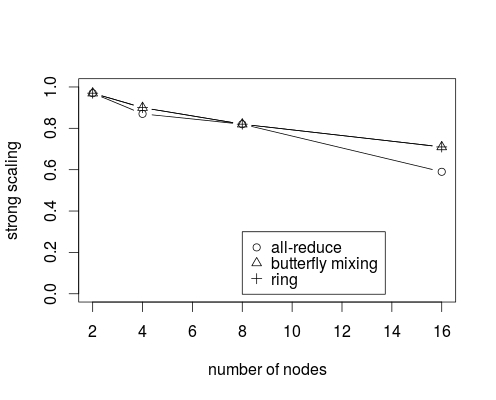
\includegraphics[width=0.5\textwidth]{strongS.jpeg}
  \caption{strong scaling}
  \label{fig:strongS}
\end{figure}
Comparing the training time of butterfly mixing with Allreduce and ring, we can find that for all cases, butterfly mixing uses less time to finish training than Allreduce, which is caused by less network communication time. For the best situation, the training time saving between butterfly mixing and Allreduce is 20\%. Even for the worest situation, the training time saving between butterfly mixing and Allreduce is 1\%. The training time between butterfly mixing and ring is relatively small: the percentage difference varies from 0.5\% to 12\%. 

\begin{table}
  \centering
  \begin{tabular}{c|c|c|c|c|c|c}
    \hline
           \multicolumn{2}{c|}{Nodes}   & 1    & 2    & 4    & 8    & 16 \\
    \hline
\multirow{3}{*}{Allreduce} &    Time    & 6.59 & 3.39 & 1.90 & 1.01 & 0.700\\
                           &    speedup & --   & 1.94 & 3.47 & 6.52 & 9.41\\
                           &strong scaling& -- & 0.97 & 0.87 &0.82 & 0.59 \\
    \hline
\multirow{3}{*}{Butterfly} &    Time    & --   & --   & 1.83 & 1.00 & 0.582\\
                           &    speedup & --   & --   & 3.60 & 6.59 & 11.32\\
                           &strong scaling&--  & --   & 0.90 & 0.82 & 0.71\\
    \hline
\multirow{3}{*}{Ring}      &    Time    & --   & --   & 1.84 & 1.01 & 0.517\\
                           &    speedup & --   & --   & 3.58 & 6.52 & 12.75\\
                           &strong scaling&--  & --   & 0.89 & 0.82 & 0.80\\
    \hline
  \end{tabular}
  \caption{Training time and speedup}
  \label{tab:speedup}
\end{table}

\subsection{Recognition results}

In this section, we apply our trained DNN to do the speech recognition to test the performance of the models. 
Table~\ref{tab:wer} illustrates the word error rate (WER) of the test results. A lower WER means the recognition results are more accurate. Since we fixed the total number of data points we used to train the DNN, there is a trade between the batch size and the synchronization. The more nodes means that for each reduction, more information is collected and averaged. However, the more nodes also means that information's asynchronization is heavier, becuase we do not communicate the weights at each update. Usually the performance of distributed system should be worse than single node. However, we find the gap between single node and distributed system is small, for some cases, the performance of distributed system is even better than single node, which means the distributed system can also get close optimal weights. \\

With increasing the number of nodes, the WER increases for all the communication strategies. When the number of nodes is 4 and 8, the WER of butterfly mixing is close to the allreduce, the WER of ring is larger than butterfly mixing. When the number of nodes is 16, the gaps among allreduce, butterfly mixing, and ring become large (but still in 10\%). In sum, the performance of DNN trained by butterfly mixing is slightly worse than that of allreduce, but better than that of ring.
\begin{table}
  \centering
  \begin{tabular}{c|c|c|c|c|c}
    \hline
    Nodes       & 1    & 2     & 4    & 8    & 16 \\
    \hline
    allreduce   & 18.4 & 17.9  & 18.3 & 18.3 & 18.7 \\
    butterfly   & --   & --    & 18.5 & 18.7 & 20.6 \\
    ring        & --   & --    & 18.5 & 19.6 & 22.1\\
    \hline
  \end{tabular}
  \caption{Word error rate on different setup}
  \label{tab:wer}
\end{table}

\section{Conclusion}
Neural network training can be efficiently speed up by using model averaging techniques.
Natural gradient method contributes to the convergence rate in model averaging setup.
Butterfly-mixing and ring reduction can reduce communication time in a further step.
Training using Butterfly-mixing and ring reduction does not converge well as the number of jobs goes up to 16.

\section{Acknowledgements}
We would like to thank Karel Vesely for who wrote the original "nnet1" neural network training code
upon which the work here is based. We would also like to thank Nelson Morgan, Forrest Iandola and Yuansi Chen
for their helpful suggestions.

% References should be produced using the bibtex program from suitable
% BiBTeX files (here: strings, refs, manuals). The IEEEbib.bst bibliography
% style file from IEEE produces unsorted bibliography list.
% -------------------------------------------------------------------------
\bibliographystyle{IEEEbib}
\bibliography{report}

\end{document}
